\chapter{Literature Review}
This review synthesizes clinical, architectural, and methodological evidence to ground our approach. We scoped sources to peer\textendash reviewed work and commonly cited practitioner guides, emphasizing fundus imaging practice and ocular disease foundations; CNN baselines and lightweight attention (SE, ECA, BAM, CBAM) alongside token\textendash based Transformers; and dataset/evaluation practices specific to ODIR\textendash 5K, including augmentation and explainability (Grad\textendash CAM, LIME/SHAP). Each strand maps directly to design: Hypertension\textendash aware labeling and patient\textendash level splits; an EfficientNet baseline with late CBAM placement for saliency control at low overhead; percent confusion matrices and macro metrics for imbalance; and Grad\textendash CAM validation that attention concentrates on clinically relevant regions. This integration underpins our hypothesis that CBAM improves separability and minority recall with modest parameter cost.

\section{Clinical and Modality Context}
A robust model must be grounded in the clinical realities and technical limitations of the data generation process. Fundus photography, while a standard diagnostic tool, is subject to numerous common pitfalls that can degrade dataset quality and, consequently, model reliability \cite{docxRef01,docxRef04,docxRef05}. These include artifacts such as camera\textendash lens dust, eyelash obstruction, poor patient fixation leading to blur, and improper illumination causing reflections or shadowed regions. Literature reviewing these practices \cite{docxRef04,docxRef05} informs the necessity of robust preprocessing and augmentation to ensure models are invariant to these non\textendash pathological variations. If not properly handled, a model might erroneously learn that an eyelash shadow is a sign of pathology, creating a ``shortcut'' feature that fails dramatically upon real\textendash world deployment.

Beyond modality artifacts, a firm clinical grounding is essential for defining class boundaries, especially given the high inter\textendash rater variability that can exist even among clinical experts. Our class definitions for Cataract and Age\textendash related Macular Degeneration (AMD) are informed by foundational literature \cite{docxRef07,docxRef08,docxRef09,docxRef12,docxRef13} that describes their expected image phenotypes. For cataracts, this primarily involves lens opacification obscuring the view of the retina, a feature the model must learn to identify. For AMD, this involves detecting key biomarkers in the macular region, such as drusen, pigmentary changes, or geographic atrophy \cite{docxRef09,docxRef12}.

Similarly, the diagnostic criteria for Hypertensive Retinopathy (H) are framed by clinical guidance \cite{docxRef14,docxRef15,docxRef16} focusing on vascular abnormalities. Our models must learn to capture subtle signs like arteriovenous (AV) nicking, copper or silver wiring of arterioles, flame\textendash shaped hemorrhages, and cotton\textendash wool spots, which are indicative of vascular damage from chronic hypertension. These signs can be subtle and often co\textendash exist with diabetic retinopathy, making a discriminative feature representation critical.

Finally, for the Myopia (M) class, we draw on references \cite{docxRef17,docxRef18} that contextualize the structural changes associated with high myopia and posterior staphyloma. These changes include significant globe elongation, which manifests in the fundus image as optic disc tilting, peripapillary atrophy, a tessellated fundus appearance, and lacquer cracks. This body of literature \cite{docxRef07,docxRef09,docxRef12,docxRef14,docxRef15,docxRef16,docxRef17,docxRef18} is critical for ensuring our model's feature extraction aligns with established clinical diagnostic criteria. This alignment is necessary to build a tool that is not just accurate, but also interpretable and trustworthy to a clinical end\textendash user.

\section{Architectures: CNNs, Transformers, and Attention}
The architectural design of a deep learning model is a primary determinant of its performance, balancing representational power with computational cost. CNNs have long been the \textit{de facto} standard in medical imaging \cite{docxRef19,docxRef20,docxRef21}, owing to strong inductive biases (spatial locality and translation invariance) that suit biomarker detection. We adopt EfficientNet \cite{tan2019efficientnet} as our CNN baseline for its state\textendash of\textendash the\textendash art accuracy\textendash efficiency trade\textendash off.

In contrast, Vision Transformers (ViT) \cite{dosovitskiy2021vit,docxRef23,docxRef24,docxRef25,docxRef26} adapt self\textendash attention to images by treating an image as a sequence of patches. ViTs offer a global receptive field and can model long\textendash range dependencies that may benefit diffuse ocular patterns. However, they often require massive pretraining and are computationally heavier than CNNs in low\textendash data settings typical of medicine.

Bridging these paradigms are attention modules that augment CNNs by helping them focus on salient signals. SE \cite{hu2018squeeze}, BAM \cite{park2018bam}, and CBAM \cite{woo2018cbam} are representative. We favor CBAM for its lightweight sequential design: first channel attention (\textit{what} to focus on), then spatial attention (\textit{where} to focus). This provides a compute\textendash efficient mechanism to refine EfficientNet features without sacrificing throughput, aiming for the best of both worlds: robust local feature extraction enhanced by attention\textendash driven selection.

\subsection{EfficientNet: Working Principle}
The core innovation of EfficientNet \cite{tan2019efficientnet} is compound scaling. Rather than scaling only one dimension (depth, width, or resolution), EfficientNet balances all three via a single coefficient \(\phi\): \(d=\alpha^{\phi}\), \(w=\beta^{\phi}\), \(r=\gamma^{\phi}\) under a compute budget. The MBConv inverted residual block forms the backbone: expand with a 1\texttimes1 conv, apply a depthwise separable conv for spatial mixing, then project with a 1\texttimes1 conv. Integrated SE attention \cite{hu2018squeeze} and Swish activations further improve efficiency and representational quality. This combination, paired with ImageNet pretraining, yields a strong, transfer\textendash effective baseline that we subsequently augment with CBAM.

\subsection{EfficientNet Architecture}
A practical overview of EfficientNet’s B0 design outlines a stem\textendash body\textendash head pipeline and details MBConv blocks with squeeze\textendash and\textendash excitation (SE), depthwise separable convolution, and swish activations \cite{tan2019efficientnet}. The B0 architecture starts with a 3\texttimes 3 stride\textendash 2 stem conv, proceeds through stages of MBConv with varying expansion ratios, kernel sizes (3\texttimes 3, 5\texttimes 5), and strides, and ends with a 1\texttimes 1 conv, global average pooling, and a fully connected classifier. This description matches our baseline configuration and motivates CBAM insertion on top of EfficientNet feature blocks.

\begin{figure}[H]
  \centering
  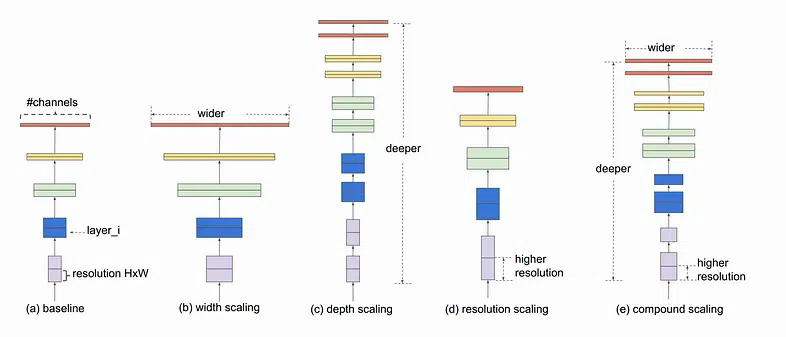
\includegraphics[width=0.92\textwidth]{../new_work/websites/Efficientnet Architecture - GeeksforGeeks_files/1_-ENqv4TI0JuyY6Nq8XQlAA.png}
  \caption{Scaling strategies summarized: individual width/depth/resolution scaling versus compound scaling that jointly balances all three.}
  \label{fig:effnet_gfg_scaling}
\end{figure}

\begin{figure}[H]
  \centering
  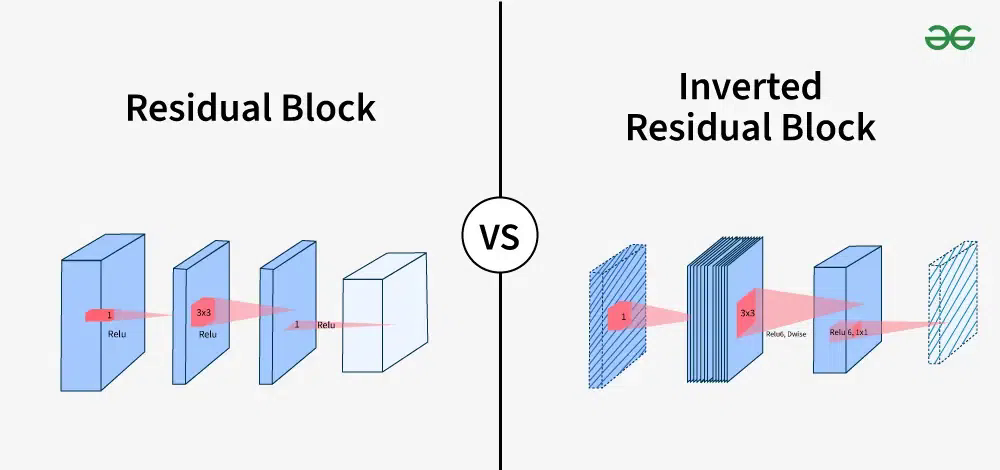
\includegraphics[width=0.92\textwidth]{../new_work/websites/Efficientnet Architecture - GeeksforGeeks_files/Residual-Block-vs-Inverted-Residual-Block.png}
  \caption{Residual vs inverted residual blocks illustrating EfficientNet’s MBConv design with depthwise separable conv and SE attention.}
  \label{fig:effnet_gfg_mbconv}
\end{figure}

\begin{figure}[H]
  \centering
  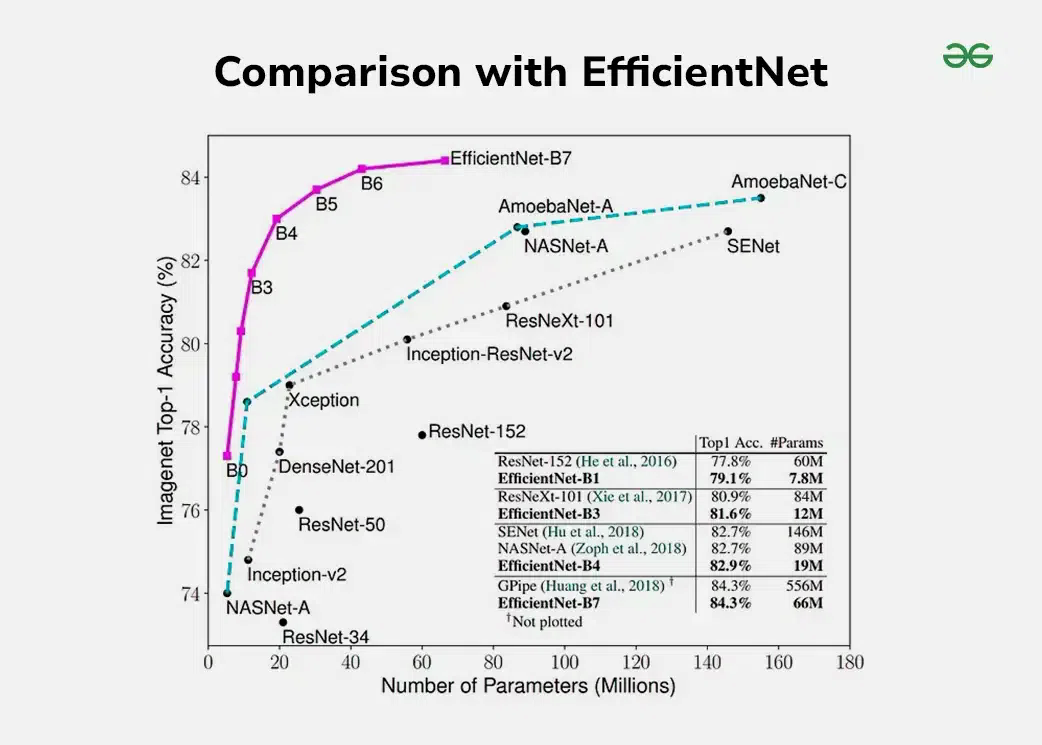
\includegraphics[width=0.92\textwidth]{../new_work/websites/Efficientnet Architecture - GeeksforGeeks_files/Comparison-with-EfficientNet-(1).png}
  \caption{Comparative positioning of EfficientNet variants by accuracy\textendash efficiency.}
  \label{fig:effnet_gfg_compare}
\end{figure}

\section{Dataset, Label Structures, and Evaluation}
We operate on ODIR\textendash 5K \cite{odir5k}, a challenging public benchmark for ocular disease classification. It is distinguished by paired left/right fundus images for 5{,}000 patients and a complex eight\textendash label structure. Its multi\textendash label nature is not an artifact but a core feature reflecting clinical comorbidity, where a single patient may present with multiple concurrent pathologies. This clinical realism makes strictly mutual\textendash exclusive losses (softmax + categorical cross\textendash entropy) ill\textendash suited. Even when a single\textendash label proxy is used (e.g., a primary diagnosis), guidance from multi\textendash label and long\textendash tailed learning \cite{docxRef62,docxRef63,docxRef64,docxRef65} remains essential: Binary Cross\textendash Entropy (BCE) treats each label as a separate binary classifier, allowing multiple positives; class re\textendash weighting and strategic sampling mitigate minority rarity.

Medical datasets are inherently long\textendash tailed; common conditions are over\textendash represented while rare but critical pathologies are scarce. This imbalance biases naive models toward majority classes. Literature on imbalance \cite{docxRef62,docxRef63} informs design choices such as inverse\textendash frequency loss weighting and careful sampling.

For evaluation, we adhere to rigorous practices in medical computer vision \cite{docxRef38,docxRef41}. The most critical protocol is patient\textendash level splitting: since the two eyes of a patient are highly correlated, splitting them across train/test induces severe leakage and inflates metrics. We confine all images from a patient to a single split (train/val/test). Beyond accuracy, we report per\textendash class precision, recall (sensitivity), F1, macro F1, and emphasize AUROC for its threshold\textendash independence and robustness under imbalance, as it measures the ability to rank positives above negatives irrespective of a fixed threshold.

\section{Data Augmentation and Synthetic Data}
To train a robust model, we teach invariances to non\textendash pathological variations common in clinical imaging. We employ geometric and photometric transforms, including random horizontal/vertical flips, small rotations (e.g., $\pm15^{\circ}$), random zooming, and brightness/contrast adjustments, simulating patient positioning and illumination variability so the model focuses on structural pathology.

Simple affine transforms are insufficient for non\textendash rigid biological tissue. We therefore incorporate elastic deformations \cite{docxRef46,docxRef47,docxRef48,docxRef49,docxRef50}, applying localized, non\textendash linear warps that better reflect subtle retinal shape changes in vivo or projection effects, forcing invariance to localized stretching/compression.

To address data scarcity in long\textendash tailed distributions, we review generative augmentation via GANs \cite{docxRef52,docxRef53,docxRef54,docxRef55,docxRef56}. The goal is targeted synthesis of rare variants to balance training; risks include mode collapse and non\textendash plausible artifacts, requiring clinical validation. Mixup/CutMix\textendash style strategies \cite{docxRef62} provide complementary regularization by blending images/labels, smoothing decision boundaries and improving calibration.

\section{Explainability and Model Interpretation}
Deep models are often criticized as ``black boxes,'' a barrier in clinical workflows where trust and accountability are paramount. We rely on Grad\textendash CAM as the primary tool: gradients into the final convolutional layer produce a coarse saliency map highlighting regions most influential for a prediction. This layer balances semantic abstraction with spatial fidelity.

Grad\textendash CAM provides clinical validation. For a correct AMD prediction, attention should concentrate on the macula (drusen, pigmentary changes); for glaucoma, activations around the optic disc indicate cupping cues. Conversely, if heatmaps highlight non\textendash pathological artifacts (e.g., eyelash shadow, lens reflection \cite{docxRef04,docxRef05}), we have identified a spurious correlation and a failure mode.

For model\textendash agnostic auditing, LIME and SHAP \cite{docxRef42,docxRef43,docxRef44,docxRef45} complement Grad\textendash CAM. LIME fits a local interpretable model around an instance via perturbations (e.g., superpixel toggling). SHAP provides game\textendash theoretic attributions (Shapley values) assigning each feature its contribution. Together they support debugging, clinician trust, and transparent communication of model decisions.

\section{Frontiers: Self\textendash Supervised and Federated Learning}
Two frontiers address fundamental medical AI bottlenecks: labeling and data access. Self\textendash supervised learning (SSL) \cite{docxRef66} reduces reliance on expert\textendash labeled datasets by learning domain representations from pretext tasks such as contrastive learning (e.g., distinguishing augmented views of the same fundus) or masked autoencoding. SSL yields pathology\textendash aware backbones that transfer better than generic ImageNet features.

Federated Learning (FL) \cite{docxRef67,docxRef68} addresses privacy, governance, and security constraints by training where the data reside: institutions train locally and share only anonymized updates for aggregation. Despite challenges (statistical heterogeneity across sites, communication costs), the synergy of SSL+FL outlines a path to scalable, privacy\textendash preserving foundation models that can be fine\textendash tuned on smaller labeled datasets.


